\subsubsection{Worker Documents, Generation and Signatures}
Document has one required Worker reference and identifies category/title/subtype;
DocumentVersion holds that worker's accepted source and version-specific metadata.
WorkerSignature binds the document worker to one reviewed version and identifies
the initiating User separately. The worker signs, not the initiating account.
Figure~\ref{fig:er-documents} shows individual document sources and signing results.
\begin{figure}[!htbp]\centering
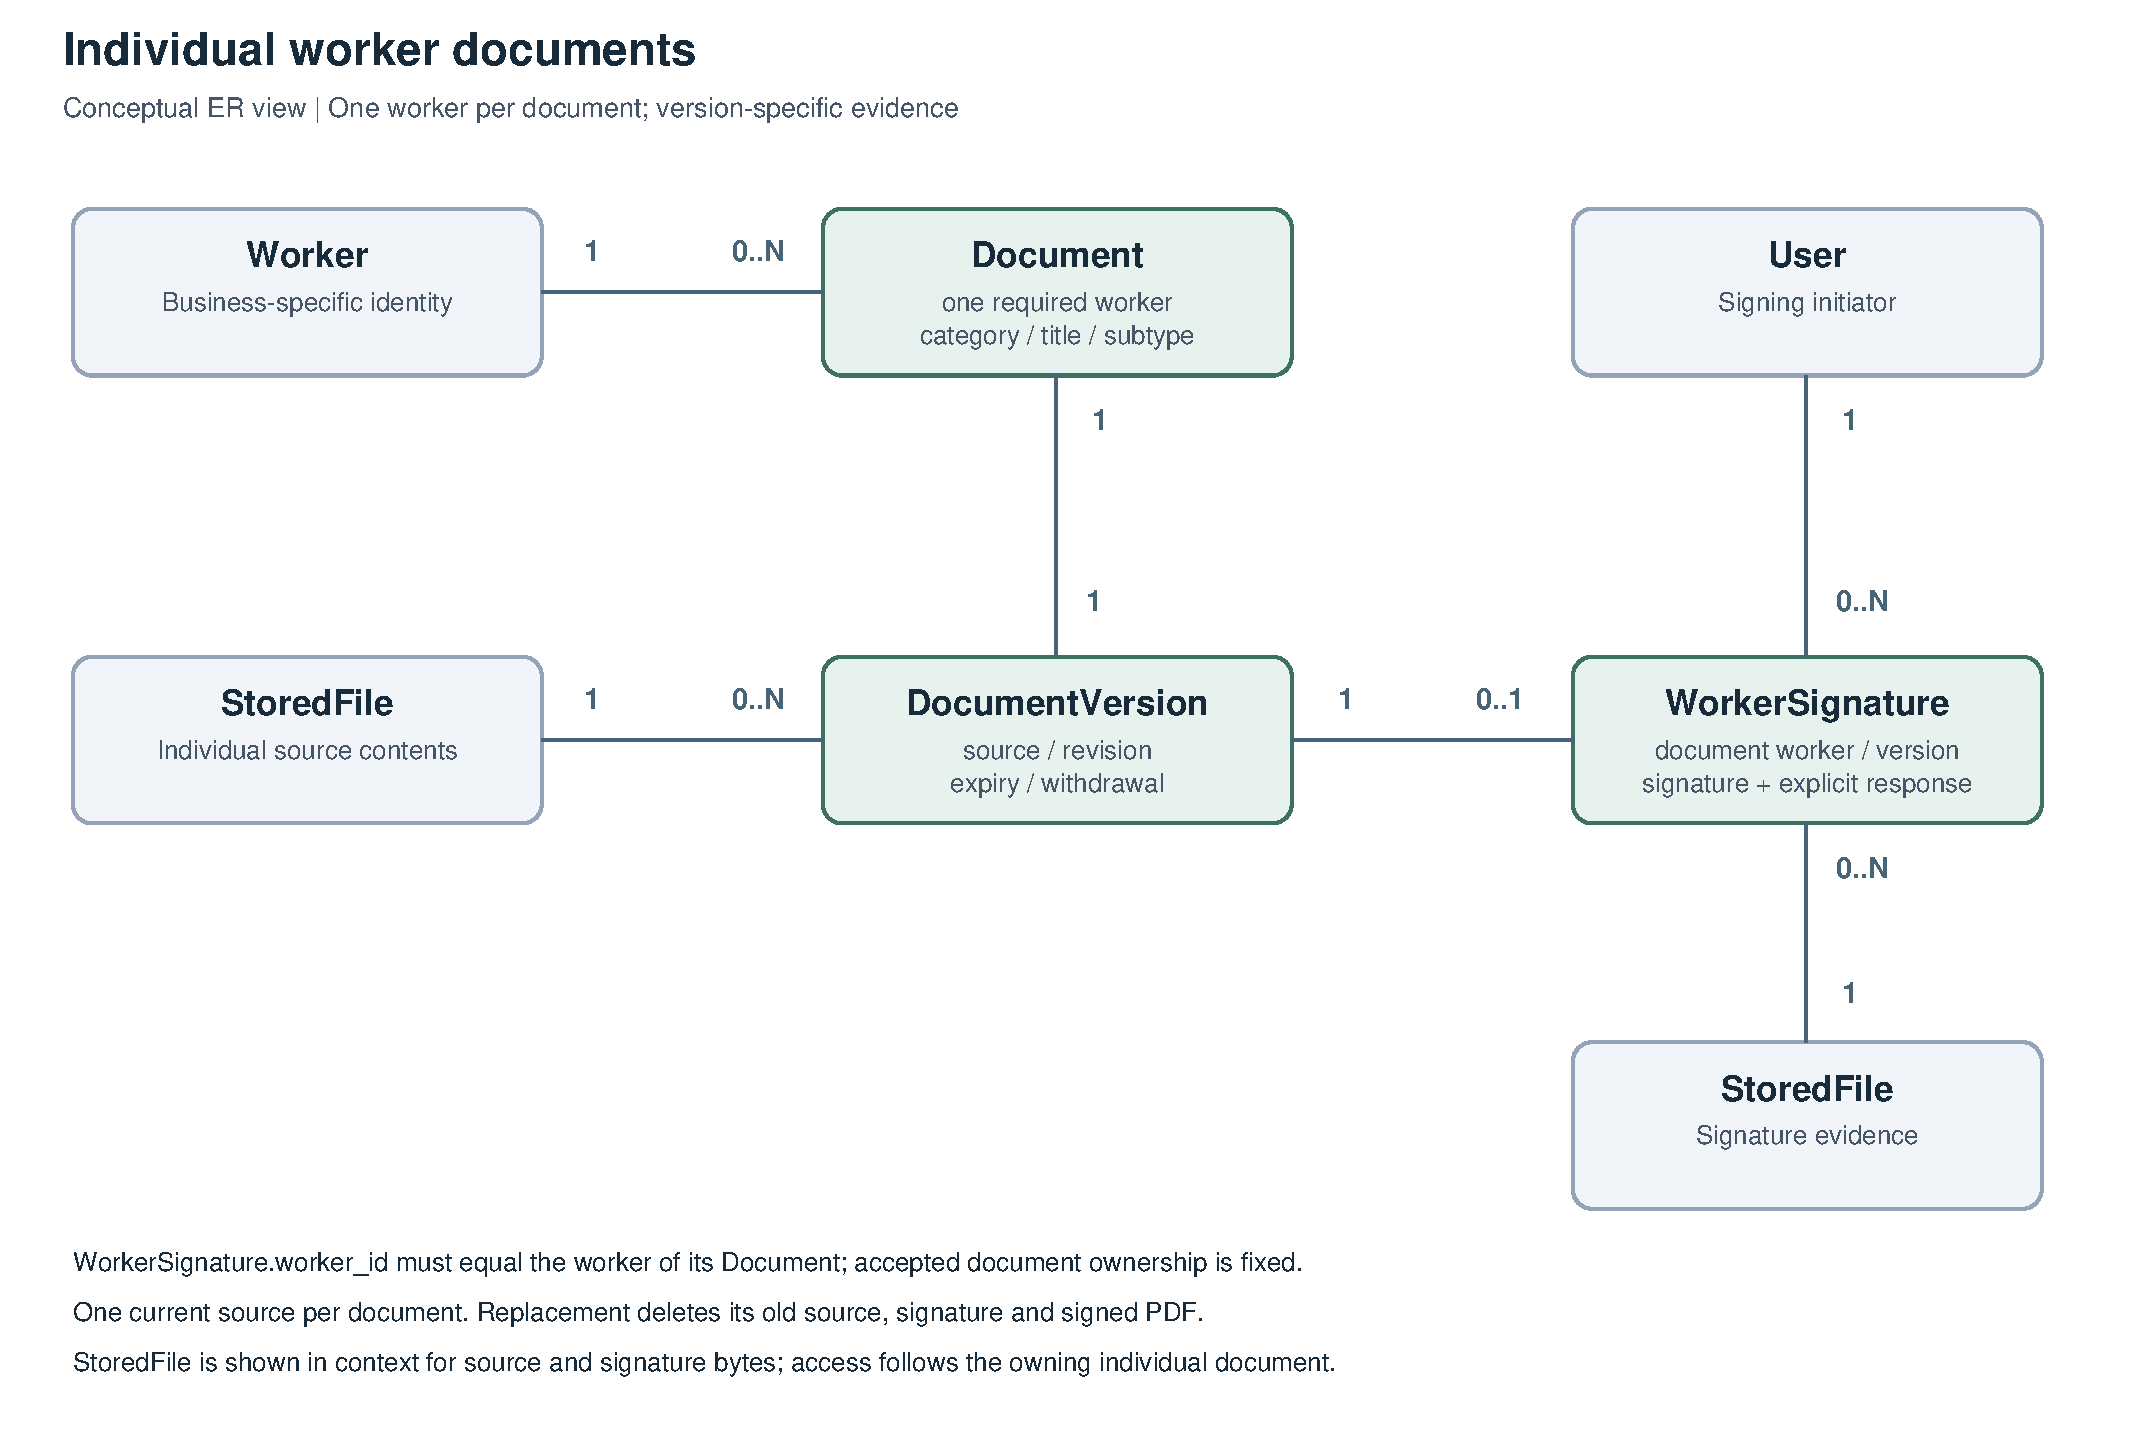
\includegraphics[width=\linewidth]{er-documents.pdf}
\caption{Individual sources and worker/version signing results. StoredFile is one entity shown in contextual views.}
\label{fig:er-documents}
\end{figure}
DocumentVersion separates source identity, currency, withdrawal, recorded expiry
and external-signature declaration. WorkerSignature records individual signing;
retention/cleanup follows \hyperref[br:026]{\identifier{BR-026}}, including deletion of a superseded source, signature and PDF and temporary recovery of ineligible signing proposals under \decisionref{Q-DOC-04}.

DocumentTemplate supplies an available model, category, revision and field schema.
Generated DocumentVersion records the template reference/revision and reviewed
input snapshot. Signing preserves that source and adds worker-specific evidence
and a derived signed PDF under \identifier{FR-042(d)}, for uploaded and generated versions alike.
DocumentRendition links a derived PDF to that version and worker. The worker-specific
rendition contains the document worker's captured signature and explicit response
where required, preserving source contents. Regeneration is not another signing event.
Figure~\ref{fig:er-generation} shows how generation and renditions relate to the source.
\begin{figure}[!htbp]\centering
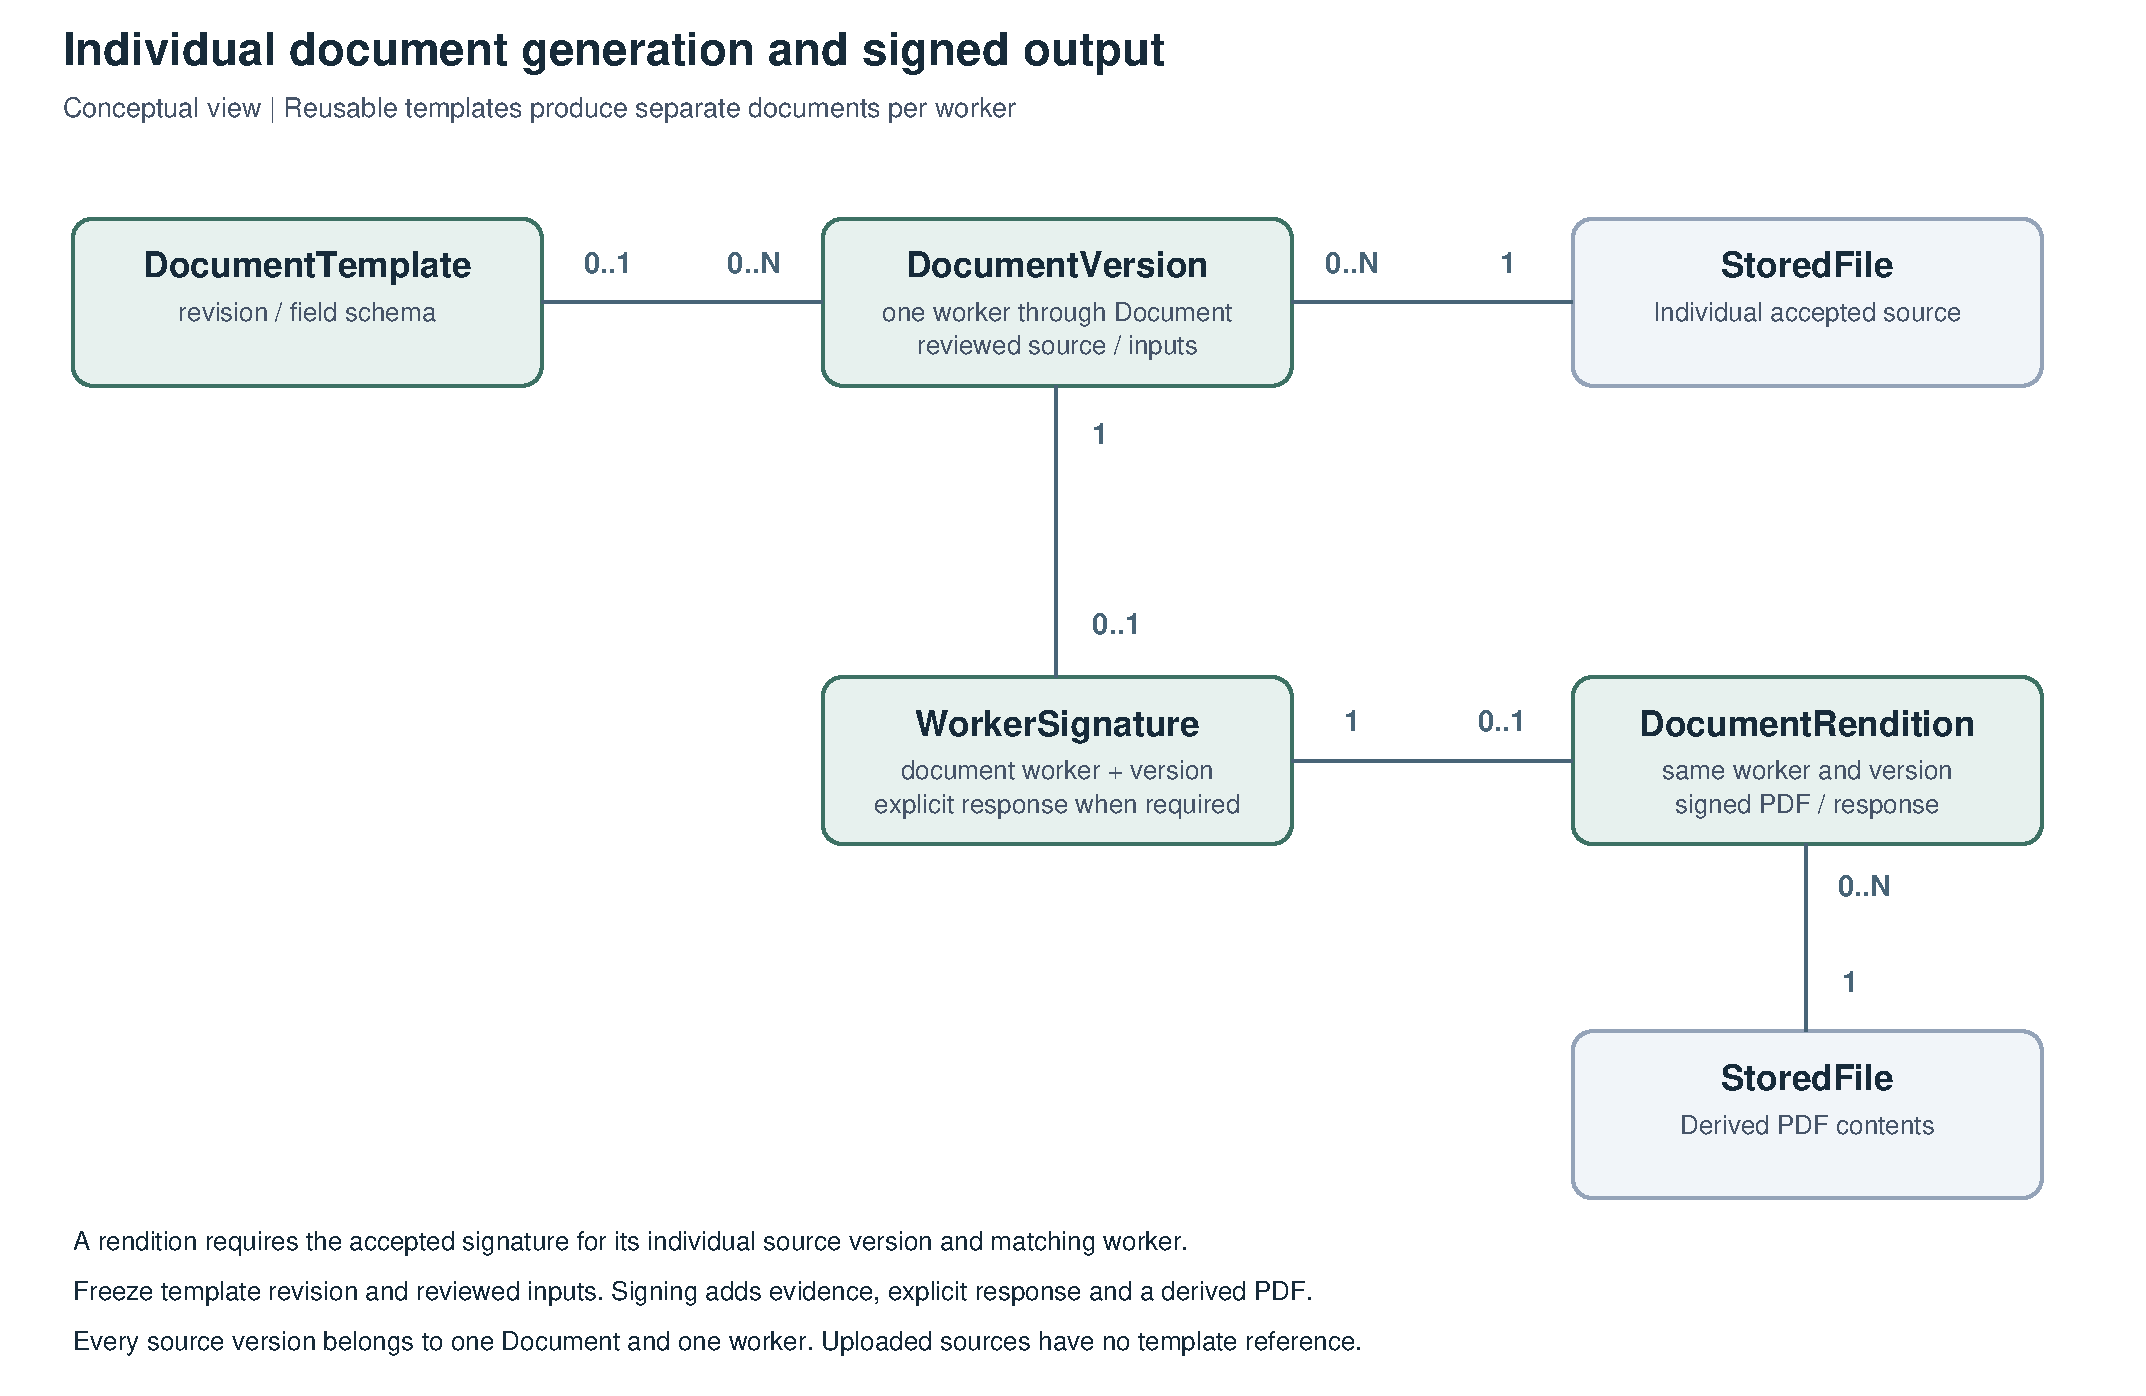
\includegraphics[width=\linewidth]{er-generation.pdf}
\caption{Template-based generation and worker-specific derived signed PDFs. Uploaded versions have no template reference.}
\label{fig:er-generation}
\end{figure}
The supplied inventory appears in Table~\ref{tab:source-forms}; the selected Spanish wording is preserved, with rendering and field mapping to be tested by the team. Document records subtype, DocumentVersion freezes source/template
inputs and any reviewed external response, and WorkerSignature binds an explicit
response to the signing event. Generation leaves consent undecided until signing;
evidence/PDF preserves the decision. Every document has one worker and one current accepted source. Replacement deletes the previous source, signature and PDF without a consultable history. Reusing a
template creates independent documents for each selected worker. Identity/permit originals are uploaded evidence; generation does not issue
them. Worker activity is derived in the profile under \identifier{FR-023}, without a dedicated attendance-document workflow. Source generation/acceptance
requires connectivity, while an accepted prepared version may be signed offline.
